\chapter{Related work}
\label{chap:related-work}

\chapter{Related and future work}










\section{Related work}
\label{sec:relwork}

A wide range of special languages have been developed to support \emph{graph based} representation and querying of computer data. A class-diagram like modeling language is Ecore of the Eclipse Modeling Framework (EMF~\cite{EMF}), where classes, references between them and attributes of classes describe the domain. Extensive tooling helps the creation and transformation of such domain models. For EMF models, OCL is a declarative constraint description and query language that can be evaluated with the local-search based Eclipse OCL~\cite{EclipseOCL} engine. To address scalability issues, impact analysis tools~\cite{OCLIA} have been developed as extensions or alternatives to Eclipse OCL.

Outside the Eclipse ecosystem, the Resource Description Framework (RDF~\cite{website:rdf_standard}) is developed to support the description of instances of the semantic web, assuming sparse, ever-growing, incomplete data. Semantic models are built up from triple statements and they can be queried using the SPARQL~\cite{SPARQL} graph pattern language with tools like Sesame~\cite{sesame} or Virtuoso~\cite{openvirtuoso}. Property graphs~\cite{DBLP:journals/corr/abs-1006-2361} provide a more general way to describe graphs by annotating vertices and edges with key-value properties. Such data structures can be stored in graph databases like Neo4j~\cite{neo4j} which provides the Cypher~\cite{cypher} query language. Even though big data storage (usually based on MapReduce) provides fast object persistence and retrieval, query engines realized directly on these data structures do not provide dedicated support for incremental query evaluation. 

In the context of event-based systems, distributed evaluation engines were proposed earlier~\cite{message-passing-rete}. However they scaled up in the number of rules \cite{mapreduce-rete} rather than in the number of data elements. As a very recent development, Rete-based caching approaches have been proposed for the processing of Linked Data (bearing the closest similarity of our approach). INSTANS~\cite{INSTANS2012} uses this algorithm to perform complex event processing (formulated in SPARQL) on RDF data, gathered from distributed sensors. Diamond~\cite{miranker2012diamond} evaluates SPARQL queries on Linked Data, but it lacks an indexing middleware layer so their main challenge is efficient data traversal.

The conceptual foundations of our approach as based on \eiq{}~\cite{models10}, a tool that evaluates graph patterns over EMF models using Rete. Up to our best knowledge, \iqd{} is the first approach to promote distributed scalability by \emph{distributed incremental query evaluation} in the MDE context. As the architecture of \iqd{} separates the data store from the query engine, we believe that the scalable processing of property graphs can open up interesting applications outside of the MDE world.


Acharya et al. described a Rete network mapping for fine grained and medium grained message-passing computers~\cite{message-passing-rete}. The medium-grained computer connected processors in a crossbar architecture, while our approach use computers connected by gigabit ethernet. The paper published benchmark results of the medium-grained solution, but these are based only on simulations.

\section{Future work}

\subsection{Cassandra}

Apache Cassandra is a mature, popular NoSQL database that stores \textit{column families} \cite{Cassandra}. Column families are similar to tables in relational databases, but have a looser schema: each row has it's set of columns.

Cassandra is fault-tolerant and highly scalable with tunable consistency properties. It's distributes the rows in the cluster using a \textit{partitioner}.

\begin{figure}
\begin{center}

\includegraphics[]{figures/cassandra-logo}
\caption{The logo of Cassandra}
\label{fig:cassandra-logo}
\end{center}
\end{figure}


\subsection{Clustered graph loader application}

The \textit{ClusterGraphLoader} application is capable of bulk loading a graph (stored in a GraphML file) to a Cassandra cluster.

The GraphML file is stored on a distributed file system, currently HDFS \cite{hadoop}. The parsing of the GraphML file is divided to to phases:

\begin{enumerate}
  \item Scan the file to determine the \texttt{<node>} and \texttt{<edge>} segments.
  \item Parse the file parallelly.
\end{enumerate}

For the second phase, we implemented a sequential GraphML parser using the Woodstox XML parser library \cite{Woodstox} which overrides the JDK's default StAX parser (\texttt{javax.xml.stream}). The second phase runs distributedly in the cluster using Akka actors and loads the nodes and edges to the Cassandra cluster. 

\subsection{Titan}

Titan is a highly scalable graph database optimized for storing and querying large graphs with billions of vertices and edges distributed across a multi-machine cluster \cite{Titan, TitanRiseOfBigData, TitanCassandra}.

Titan supports various storage backends, including Apache Cassandra \cite{Cassandra} and Apache HBase \cite{HBase}. Unlike disk-based graph databases (e.g.\ Neo4j), Titan offers horizontal scalability and sharding of graphs.

\begin{figure}
\begin{center}
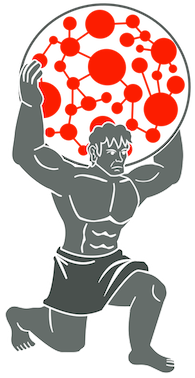
\includegraphics[]{figures/titan-logo}
\caption{The logo of Titan}
\label{fig:titan-logo}
\end{center}
\end{figure}

For our experiments, we used Cassandra as the storage backend because of it's easy deployment and great tunability.

\subsubsection{Titan and Cassandra setups}

In order to use Gremlin's full processing power, we have to use Rexster, a graph server that exposes any Blueprints graph through REST \cite{Rexster}.

Titan, Cassandra and Rexster can be deployed in two different setups: remote server mode(\autoref{fig:titan-modes-rexster}) and the embedded mode (\autoref{fig:titan-modes-embedded}).

\begin{figure}
\begin{center}
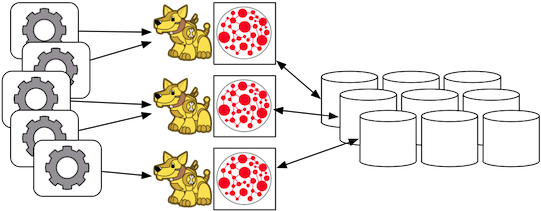
\includegraphics[width=10cm]{figures/titan-modes-rexster}
\caption{Titan's remote server mode}
\label{fig:titan-modes-rexster}
\end{center}
\end{figure}

\begin{figure}
\begin{center}
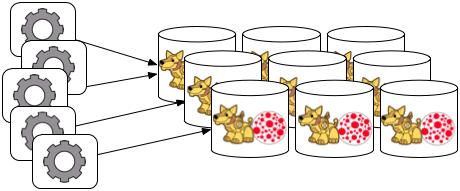
\includegraphics[width=10cm]{figures/titan-modes-embedded}
\caption{Titan's embedded mode}
\label{fig:titan-modes-embedded}
\end{center}
\end{figure}

\subsubsection{Initialising Titan}

\begin{lstlisting}[caption=Gremlin commands to initialize the a single-node Titan instance, label=lst:titan-singlenode, breaklines=true]
g = TitanFactory.open('mygraphdir');
g.createKeyIndex("idx", Vertex.class);
g.createKeyIndex("type", Vertex.class);
g.loadGraphML('/home/szarnyasg/data/testBig_User_1.graphml');
\end{lstlisting}

\subsubsection{Listing nodes}

The Gremlin code to list all \texttt{ROUTE\_ROUTEDEFINITION} edges is shown in \autoref{lst:gremlin-route-routedefinition} (see also the Cypher query in \autoref{lst:cypher-route-routedefinition})

\begin{figure}
\begin{center}
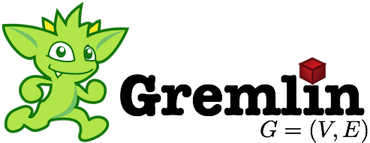
\includegraphics[]{figures/gremlin-logo}
\caption{The logo of Gremlin}
\label{fig:gremlin-logo}
\end{center}
\end{figure}

\begin{lstlisting}[caption=Gremlin query to retrieve all \texttt{ROUTE\_ROUTEDEFINITION} edges, label=lst:gremlin-route-routedefinition, breaklines=true]
t = new Table(); 
g.idx('node_auto_index')[[type:'Route']].as('Route').outE('ROUTE_ROUTEDEFINITION').as('RouteDefinition').inV.as('Sensor').table(t).iterate();
t;
\end{lstlisting}
